% !TeX program = xelatex
% !TeX encoding = UTF-8
% !TeX TXS-program:compile = "D:/texlive/2025/bin/windows/xelatex.exe" -synctex=1 -interaction=nonstopmode %.tex
\documentclass[UTF8,a4paper,11pt,fontset=windows]{ctexart}
\usepackage[left=25mm,right=25mm,top=24mm,bottom=25mm]{geometry}
\usepackage{amsmath,amssymb,graphicx,booktabs,longtable,array,caption,enumitem}
\usepackage[hidelinks]{hyperref}
\setmainfont{Times New Roman}
\setmonofont{Consolas}
\linespread{1.22}
\setlength{\parindent}{2em}
\setlength{\emergencystretch}{2em}
\setlength{\LTpre}{6pt}
\setlength{\LTpost}{10pt}
\setlist{nosep,topsep=5pt}
\captionsetup{font=small,labelfont=bf,labelsep=quad}
\ctexset{section={format=\Large\bfseries},subsection={format=\large\bfseries},subsubsection={format=\normalsize\bfseries}}
\hypersetup{pdftitle={EquiAffect-3B：基于类别感知监督策略优化的多模态行为分类模型},pdfsubject={中文论文初稿}}
\title{EquiAffect-3B：基于类别感知监督策略优化的多模态行为分类模型}
\author{}
\date{中文初稿 v0.6\quad 2026年10月8日}
\begin{document}
\maketitle

\begin{abstract}

多模态行为分类需要模型同时利用不同输入线索并区分多个类别，但策略优化中的有效学习信号并不总能覆盖真实标签。组内奖励塌缩会削弱相对优势，而仅调整已有回答的优势尺度，也难以直接约束主导类别的过度预测。针对这一问题，本文提出类别感知监督策略优化（Class-Aware Supervised Policy Optimization，CALSPO），并基于Qwen2.5-Omni-3B训练得到多模态行为分类模型EquiAffect-3B。该方法以HARPO为基础，将AVSPO的优势恢复适配到连续复合奖励，在恢复后的真实回答优势上进行异质性调制，并加入按训练类别频数加权的真实标签监督。实验覆盖情绪分类与抑郁分类两个任务。在328题评估集上，EquiAffect-3B的整体正确率由HARPO的59.76\%提高至65.55\%，情绪Macro-F1由55.03\%提高至62.91\%，非中性误判为中性的比例由27.24\%降至19.51\%。同时，中性召回率100\%对应46.07\%的精确率，文本与音频子集的中性文本倾向达到86.41\%。本文同时提供CALSPO方法实现与EquiAffect-3B训练后LoRA权重。结果表明，该模型在本次评估中改善了分类表现并减轻了中性偏向，但主导类别过度预测与格式问题仍然存在。代码与模型权重将于终版投稿时在仓库\url{https://github.com/zhe293/CALSPO}公开。

\par\medskip\noindent \textbf{关键词：} 多模态行为分类；EquiAffect-3B；CALSPO；类别偏向；标签监督
\end{abstract}

\section{引言}

多模态行为分类通过文本、语音和视觉线索识别情绪及其他行为状态。MultiEMO研究不同模态之间的关联与情绪类别区分\cite{ref1}，Emotion-LLaMA利用指令微调开展多模态情绪识别与推理\cite{ref2}。Human Behavior Atlas将多种心理与社会行为任务组织为统一基准\cite{ref3}，AffectGPT进一步扩展了描述性情绪理解与自然语言输出评价\cite{ref4}。不同任务的标签空间、输入模态与类别分布存在差异，使模型需要在共享参数中学习多种判别目标。

类别分布不均衡可能使学习偏向高频标签\cite{ref5}，对话情绪识别研究也已讨论标签、说话人与词语关联带来的预测偏向\cite{ref6}。Wang等指出，不平衡的语音情绪数据可能使模型过拟合占多数的中性类别\cite{ref25}。强化学习可以利用生成答案的反馈优化策略，但整体性能提升并不意味着各类别得到均衡识别：模型可能频繁输出某一主导类别，同时将其他类别吸收到该预测中。本文将这种预测现象称为类别偏向，并以情绪分类中的中性过度预测作为具体研究对象。

组相对策略优化（GRPO）通过同题多个回答的奖励统计构造相对优势\cite{ref7}。HARPO进一步根据优势幅值的贡献代理量，在问题与任务层面调节学习信号，以处理行为数据的异质性\cite{ref8}。这些方法主要作用于模型已经生成的回答。当同题奖励相同，相对优势可能退化为零；即使借助虚拟奖励恢复更新方向\cite{ref9}，全错组仍缺少正确类别的直接学习目标。因此，奖励塌缩恢复与标签约束是需要分别处理的两个环节。

为此，本文提出CALSPO，将连续复合奖励下的优势恢复、HARPO调制和类别加权标签监督接入同一优化过程，并以该方法训练EquiAffect-3B。强化学习分支保留对真实生成回答的策略更新，监督分支则对每个训练问题提供真实标签目标，并根据训练频数调节不同类别的损失权重。本文将算法与训练所得模型共同作为研究产出，提供CALSPO实现及EquiAffect-3B训练后LoRA权重；在匹配主要训练条件的HARPO基线上检验该模型的表现，并同时观察类别误判与无效输出，以判断指标改善是否伴随偏向减轻。

本文的主要工作包括：

\begin{enumerate}
\item 提出CALSPO，将AVSPO优势恢复适配到连续复合奖励，并结合HARPO调制与类别加权标签监督构建联合优化目标。
\item 开发EquiAffect-3B，以共享模型联合处理情绪与抑郁分类，并提供训练后LoRA适配权重、基座版本及加载说明。
\item 在情绪与抑郁分类任务上比较EquiAffect-3B与HARPO训练基线，并结合逐类指标、混淆矩阵及无效答案，分析中性偏向的改善及剩余偏向与输出问题。
\end{enumerate}

\section{相关工作}

\textbf{组相对策略优化与奖励塌缩。} GRPO使用同题回答组的奖励均值与标准差计算相对优势\cite{ref7}。当组内奖励相同，相对优势可能归零。已有方法从不同环节补充学习信号：DAPO通过动态采样筛除回答全部正确或全部错误的问题组，并继续采样\cite{ref10}；AVSPO加入自适应虚拟奖励参照\cite{ref9}；NGRPO结合虚拟最高奖励参照与非对称裁剪处理全错组\cite{ref11}；SGPO则通过步骤判别反馈区分错误推理\cite{ref12}。CALSPO采用AVSPO的统计恢复思路，将其适配到连续复合奖励，并保留真实回答用于策略更新。

\textbf{异质性感知的行为学习。} OmniSapiens利用HARPO调制问题与任务层面的优势，以应对不同输入及任务产生的学习信号差异\cite{ref8}。其调制依据为绝对优势构造的贡献代理，而非直接测量参数梯度。CALSPO保留这一优势调制主线，并将其输入替换为恢复后的真实回答优势。

\textbf{标签监督与策略更新。} 监督目标与策略优化的联合已有研究基础。InstructGPT的PPO-ptx在强化学习更新中混入预训练似然目标，以减轻其他任务上的性能退化\cite{ref13}；SRFT通过熵感知权重，将示范监督与自采样回答的强化学习接入单阶段微调\cite{ref14}。CALSPO关注多模态行为分类，为同一输入提供真实标签及必要格式的监督，与恢复及调制后的策略优势共同优化；其辅助目标不包含人工推理链，采用训练频数类别权重和固定辅助系数。

\textbf{类别不平衡与重加权。} Wang等针对多数中性类过拟合问题，结合原始语音与潜在表示层的Mixup增强学习情绪表示\cite{ref25}。这项工作表明，中性类别偏向已有研究基础；其重点是语音增强与表示学习，而本文研究生成式多模态分类中的策略更新与类别加权标签监督。Class-Balanced Loss利用有效样本数重新加权监督损失\cite{ref5}，Focal Loss通过降低易分类样本的损失贡献，使训练更关注难例\cite{ref15}。Logit调整依据类别频率修正分类得分\cite{ref16}，Balanced Softmax则在分类归一化中考虑训练与测试标签分布的差异\cite{ref17}。CALSPO采用训练频数反平方根构造静态类别权重，将其用于生成式标签监督；这一权重不同于有效样本数或预测难度权重，也不修改推理阶段的类别logit。

\textbf{多模态情绪理解与去偏。} MulT通过跨模态注意力建模不同模态序列之间的关联\cite{ref18}，MultiEMO进一步关注对话情绪融合及少数、语义相近类别的区分\cite{ref1}。生成式路线中，Emotion-LLaMA融合情绪编码与指令微调\cite{ref2}，AffectGPT面向描述性情绪理解建立模型、数据和评价基准\cite{ref4}。TFD通过预测阶段的反事实推理处理对话情绪识别中的数据偏向\cite{ref6}。本文使用已有多模态基座，重点研究训练目标中的类别学习信号，采用固定标签匹配和无效输出统计评价分类表现。

\section{EquiAffect-3B模型与CALSPO训练方法}

\subsection{模型与任务设置}

EquiAffect-3B采用Qwen2.5-Omni-3B\cite{ref19}作为多模态基座，以CALSPO通过一个共享模型联合训练情绪分类和抑郁分类。输入可包含文本、音频与视频。情绪标签为愤怒、厌恶、恐惧、高兴、中性、悲伤和惊讶；抑郁分类包含抑郁与非抑郁两类。训练时冻结基座参数，只更新LoRA适配参数\cite{ref20}。

EquiAffect-3B是经CALSPO训练得到的模型名称，CALSPO是其训练算法；模型沿用基座架构。训练所得权重以LoRA适配器形式交付，与固定版本的基座共同加载，权重及版本记录见附录D。

CALSPO包含策略更新和标签监督两个分支。策略分支对每个问题生成G个真实回答，依次进行奖励计算、优势恢复、HARPO调制与策略损失计算；监督分支为每个问题构造一个真实标签目标。两个分支在同一优化步骤中累积梯度。完整流程见附录A.1。

\subsection{预备知识}

设问题为q，其任务为m，策略$\pi_\theta$生成回答组，其归一化奖励为$r_i$。按本地实现，普通组相对优势为：

\begin{equation}
a_i=\frac{r_i-\mu_q}{\max(\sigma_q,\varepsilon)}\label{eq:1}
\end{equation}

其中$\mu_q$和$\sigma_q$为该组真实奖励的均值与总体标准差。当$\sigma_q$接近零，优势缺少有效差异。另一方面，不同问题与任务的优势尺度可能不同。CALSPO先处理组内奖励塌缩，再利用HARPO调节恢复后的优势幅值。

\subsection{CALSPO优化机制}

\subsubsection{连续复合奖励下的优势恢复}

本文采用AVSPO的虚拟奖励参照思想\cite{ref9}。格式与长度项使组内奖励不仅由标签正确性决定。因此，CALSPO分别判断奖励塌缩和回答是否全部正确或全部错误。当批次塌缩率超过动态阈值，且某组同时满足奖励塌缩与全对或全错条件时，将虚拟奖励加入该组的统计参照。

对全错塌缩组，虚拟奖励高于真实奖励锚点；对全对塌缩组，虚拟奖励低于该锚点。利用真实与虚拟奖励的联合均值$\mu_{\mathrm{aug}}$和总体标准差$\sigma_{\mathrm{aug}}$，仅对真实回答计算：

\begin{equation}
a_i=\frac{r_i-\mu_{\mathrm{aug}}}{\max(\sigma_{\mathrm{aug}},\varepsilon)}\label{eq:2}
\end{equation}

由此，全错塌缩组的真实回答获得负优势，全对塌缩组获得正优势。虚拟奖励改变统计参照，不生成新文本，也不直接参与模型梯度计算。触发条件、虚拟奖励数及阈值更新见附录A.2。

\subsubsection{恢复后优势的异质性调制}

CALSPO沿用HARPO的绝对优势贡献代理\cite{ref8}，先在同任务问题间构造几何参照，得到问题尺度$s_q$，再对本批出现的任务构造任务尺度$s_m$。最终优势为：

\begin{equation}
A_i=a_i\,s_q\,s_m\label{eq:3}
\end{equation}

问题层尺度由当前批次计算；任务层对密度和对数尺度进行惯性平滑。本文实现的问题尺度截断至[0.5,3.0]，任务尺度截断至[0.5,4.0]，任务层两项EMA旧值系数均为0.75。各回答的有效生成token共享其优势。具体计算和状态初始化见附录A.3。

\subsubsection{类别加权标签监督}

优势恢复为已生成回答提供更新方向，真实标签监督则补充应当输出的类别。CALSPO按问题唯一标识对回答组去重，为每个原始问题构造一次“方框中的真实标签＋序列结束符”目标，输入保持相同的多模态内容。

将目标分为标签内容与格式及结束符两部分。设相应平均负对数似然分别为$L_{\mathrm{label}}$和$L_{\mathrm{format}}$，则：

\begin{equation}
L_{\mathrm{target}}(q)=L_{\mathrm{label}}(q)+0.5L_{\mathrm{format}}(q)\label{eq:4}
\end{equation}

类别重加权可用于调整监督损失中的类别贡献\cite{ref5}。本文的类别权重仅根据训练频数确定。任务m有$N_m$个问题、标签集合$C_m$，第c类频数为$n_{mc}$；以频数反平方根构造权重，经任务内样本加权均值$Z_m$归一化并截断：

\begin{equation}
w_{mc}=\operatorname{clip}\!\left(\frac{\sqrt{N_m/(|C_m|n_{mc})}}{Z_m},\,0.5,\,2.0\right)\label{eq:5}
\end{equation}

本次训练中，中性标签的监督权重为0.7204，其余情绪类别为1.0188至1.3222。该设计对高频类别降低辅助损失权重，并保留低频类别的直接监督。对Q个去重问题取平均：

\begin{equation}
L_{\mathrm{aux}}=\frac{1}{Q}\sum_q w_{mc}L_{\mathrm{target}}(q)\label{eq:6}
\end{equation}

标签监督覆盖每个训练问题，独立于优势恢复的触发状态。目标构造、token识别和完整权重见附录A.4。

\subsubsection{联合目标}

CALSPO沿用PPO式裁剪策略损失\cite{ref21}，并加入类别加权标签监督：

\begin{equation}
L=L_{\mathrm{policy}}+\lambda L_{\mathrm{aux}},\qquad\lambda=1.0\label{eq:7}
\end{equation}

策略分支使用经恢复与调制的优势$A_i$，监督分支使用真实标签目标。联合计算不训练独立critic，当前配置省略显式KL奖励与KL损失。裁剪参数及损失归约见附录A.5。

\subsection{奖励设计}

本文沿用HARPO的正确性、格式与长度组合奖励\cite{ref8}。对回答i，定义：

\begin{equation}
R_i=0.8y_i+0.2f_i+0.75p(L_i)\label{eq:8}
\end{equation}

\textbf{正确性。} $y_i$为最终标签是否精确匹配真实标签的二值奖励。

\textbf{格式。} $f_i$为回答是否满足思考段及方框答案结构的二值奖励。

\textbf{长度。} p($L_i$)在回答长度不超过192 token时为0，随后线性下降，在256 token时达到$-$1。

将全部真实回答的复合奖励在当前批内归一化后，执行第3.3节的优势计算。HARPO与CALSPO采用相同奖励实现；详细归一化和长度边界见附录A.2。

\section{实验}

本文使用Human Behavior Atlas\cite{ref3}的两个分类任务子集，比较HARPO训练基线与采用CALSPO训练的EquiAffect-3B。训练集包含304题，评估集包含328题，其中情绪分类287题、抑郁分类41题。两种方法使用相同的Qwen2.5-Omni-3B基座、训练数据、LoRA设置和奖励，均评估第38步检查点。学习率为1$\times$$10^{-6}$，优化器为AdamW\cite{ref22}，每题生成4个训练回答。为便于比较训练方法，后文表格与图中的“CALSPO”均指EquiAffect-3B，“HARPO”指采用HARPO训练的基线模型。完整数据与参数见附录B。

本文报告正确率、Macro-F1、逐类精确率与召回率，以及无效输出率；结果均采用百分制。无法精确匹配合法标签的答案计为无效，并保留在错误及完整分母中。本研究采用单标签分类指标，不将其与原论文的情绪加权准确率或抑郁加权F1混同。实验围绕三个问题展开：

\begin{itemize}
\item \textbf{RQ1：} CALSPO相较HARPO能否改善整体及分任务分类表现？
\item \textbf{RQ2：} 这种改善是否伴随主导类别误判的减少？
\item \textbf{RQ3：} 剩余偏向和无效输出集中在哪些输入条件？
\end{itemize}

\subsection{分类性能比较}

\textbf{RQ1。} 表1显示，CALSPO的整体正确率由59.76\%提高至65.55\%，增加5.79个百分点。收益主要来自情绪分类，正确率提高6.62个百分点，Macro-F1由55.03\%提高至62.91\%。抑郁分类的两项指标保持一致，未观察到额外收益。


\begingroup
\small
\setlength{\tabcolsep}{4pt}
\renewcommand{\arraystretch}{1.22}
\noindent\begin{minipage}{\linewidth}
\centering
\captionof{table}{分类表现（\%）。 两种方法评估相同题目。整体正确率按全部328题计算；情绪和抑郁指标分别以287题、41题计算。F1采用百分制显示。}\label{tab:1}
\begin{tabular}{>{\raggedright\arraybackslash}p{\dimexpr 0.23\linewidth-11.04pt\relax}>{\raggedright\arraybackslash}p{\dimexpr 0.154\linewidth-7.392pt\relax}>{\raggedright\arraybackslash}p{\dimexpr 0.154\linewidth-7.392pt\relax}>{\raggedright\arraybackslash}p{\dimexpr 0.154\linewidth-7.392pt\relax}>{\raggedright\arraybackslash}p{\dimexpr 0.154\linewidth-7.392pt\relax}>{\raggedright\arraybackslash}p{\dimexpr 0.154\linewidth-7.392pt\relax}}
\toprule
\textbf{方法} & \textbf{整体正确率} & \textbf{情绪正确率} & \textbf{情绪Macro-F1} & \textbf{抑郁正确率} & \textbf{抑郁Macro-F1} \\
\midrule
HARPO & 59.76\% & 54.36\% & 55.03\% & 97.56\% & 96.80\% \\
CALSPO & 65.55\% & 60.98\% & 62.91\% & 97.56\% & 96.80\% \\
\bottomrule
\end{tabular}
\end{minipage}
\par\medskip
\endgroup

\subsection{类别偏向分析}

\textbf{RQ2。逐类表现。} CALSPO在多个情绪类别上提高召回率和F1（表2）。恐惧召回率由19.51\%提高至29.27\%，悲伤由24.39\%提高至36.59\%，但仍低于愤怒与中性。混淆矩阵进一步显示，多个非中性类别仍被预测为中性（图1）。


\begingroup
\small
\setlength{\tabcolsep}{4pt}
\renewcommand{\arraystretch}{1.22}
\noindent\begin{minipage}{\linewidth}
\centering
\captionof{table}{逐类情绪指标（\%）。 P、R分别表示精确率和召回率；各真实类别样本量均为41。}\label{tab:2}
\begin{tabular}{>{\raggedright\arraybackslash}p{\dimexpr 0.13\linewidth-7.28pt\relax}>{\raggedright\arraybackslash}p{\dimexpr 0.145\linewidth-8.12pt\relax}>{\raggedright\arraybackslash}p{\dimexpr 0.145\linewidth-8.12pt\relax}>{\raggedright\arraybackslash}p{\dimexpr 0.145\linewidth-8.12pt\relax}>{\raggedright\arraybackslash}p{\dimexpr 0.145\linewidth-8.12pt\relax}>{\raggedright\arraybackslash}p{\dimexpr 0.145\linewidth-8.12pt\relax}>{\raggedright\arraybackslash}p{\dimexpr 0.145\linewidth-8.12pt\relax}}
\toprule
\textbf{类别} & \textbf{HARPO P} & \textbf{HARPO R} & \textbf{HARPO F1} & \textbf{CALSPO P} & \textbf{CALSPO R} & \textbf{CALSPO F1} \\
\midrule
愤怒 & 75.00\% & 87.80\% & 80.90\% & 80.00\% & 87.80\% & 83.72\% \\
厌恶 & 88.24\% & 36.59\% & 51.72\% & 85.00\% & 41.46\% & 55.74\% \\
恐惧 & 61.54\% & 19.51\% & 29.63\% & 80.00\% & 29.27\% & 42.86\% \\
高兴 & 72.22\% & 63.41\% & 67.53\% & 73.68\% & 68.29\% & 70.89\% \\
中性 & 36.19\% & 92.68\% & 52.05\% & 46.07\% & \textbf{100.00\%} & 63.08\% \\
悲伤 & 66.67\% & 24.39\% & 35.71\% & 83.33\% & 36.59\% & 50.85\% \\
惊讶 & 85.19\% & 56.10\% & 67.65\% & 86.67\% & 63.41\% & 73.24\% \\
\bottomrule
\end{tabular}
\end{minipage}
\par\medskip
\endgroup

\begin{center}
\begin{minipage}{\linewidth}
\centering
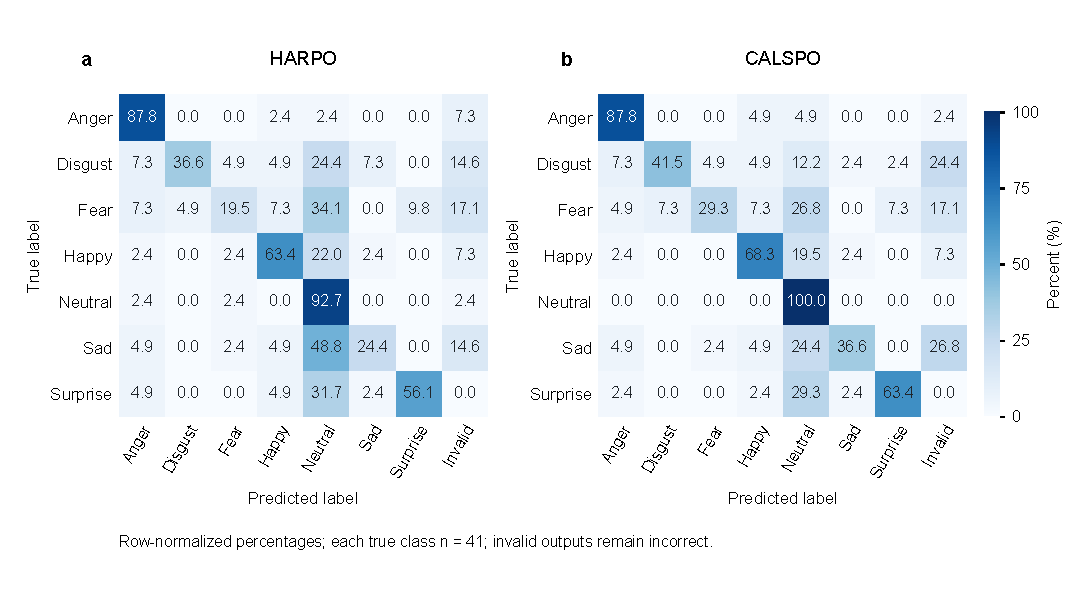
\includegraphics[width=\linewidth]{figures/fig1_confusion.pdf}
\captionof{figure}{情绪分类误判结构。 a，HARPO；b，CALSPO。行、列分别为真实类别和预测类别，最后一列保留无效输出；各行按该真实类别的全部样本归一化为百分比，两面板共用0—100\%色阶。情绪样本量n=287，各真实类别n=41。}\label{fig:1}
\end{minipage}
\end{center}

\textbf{中性召回与过度预测。} CALSPO的中性召回率达到100\%，精确率为46.07\%，即其有效中性预测中53.93\%属于其他真实类别。中性真实占比为14.29\%，有效中性预测占比为31.01\%。这表明，100\%中性召回与一定程度的过度预测同时存在，需结合精确率评价其识别表现。

\textbf{偏向变化。} 相较HARPO，CALSPO的非中性误判为中性的比例由27.24\%降至19.51\%，降低7.72个百分点；有效中性预测占比由36.59\%降至31.01\%。若计入以“neutral”开头的无效文本，情绪回答的中性倾向比例由44.25\%降至41.81\%。两种口径均反映出中性偏向减轻，而有效中性预测与输出文本倾向的改善幅度有所不同。

\subsection{输入条件与输出有效性}

\textbf{RQ3。中性倾向的集中分布。} 在文本与音频子集中，CALSPO的有效中性预测占比为56.31\%，高于18.45\%的真实中性占比，中性精确率为32.76\%。该子集的无效答案均以“neutral”开头；连同有效中性预测，86.41\%的输出呈现中性倾向，HARPO的对应比例为88.35\%（图2）。对该子集的真实非中性问题，CALSPO有83.33\%的输出表现出这一倾向。相比之下，三模态子集的中性精确率为70.97\%。

\begin{center}
\begin{minipage}{\linewidth}
\centering
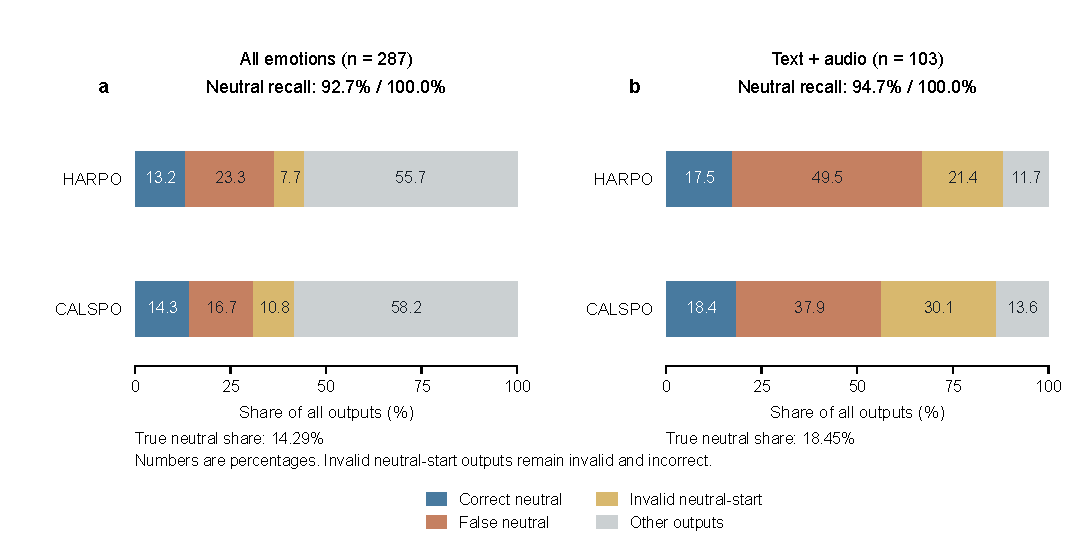
\includegraphics[width=\linewidth]{figures/fig2_neutral_bias.pdf}
\captionof{figure}{中性预测与无效文本的分解。 a，全体情绪问题；b，文本与音频子集。横条区分正确中性预测、非中性误判、以“neutral”开头的无效答案及其他输出。横轴和段内数字均为百分比，分母分别为287题和103题；显示值保留一位小数，舍入后总和可能略偏离100\%。标题的中性召回按HARPO、CALSPO顺序列出，分母为对应范围的真实中性样本。前缀统计仅用于文本诊断，无效答案仍按错误处理。}\label{fig:2}
\end{minipage}
\end{center}

\textbf{分类表现与输出有效性。} CALSPO在三模态子集的正确率由69.57\%提高至77.72\%，无效输出率由1.63\%降至0.54\%。文本与音频子集的正确率由27.18\%提高至31.07\%，无效输出率由22.33\%升至30.10\%（表3、图3）。总体情绪无效输出率由9.06\%升至11.15\%，其中96.88\%来自文本与音频子集。高兴与惊讶在该子集的严格召回率仍为0.00\%。这些结果表明，分类收益与输出有效性的变化因输入条件和类别而异。


\begingroup
\small
\setlength{\tabcolsep}{4pt}
\renewcommand{\arraystretch}{1.22}
\noindent\begin{minipage}{\linewidth}
\centering
\captionof{table}{不同输入条件的正确率与无效输出率（\%）。 无效答案保留在各子集的完整分母中。纯文本对应抑郁任务；分模态Macro-F1见附录C。}\label{tab:3}
\begin{tabular}{>{\raggedright\arraybackslash}p{\dimexpr 0.23\linewidth-11.04pt\relax}>{\raggedright\arraybackslash}p{\dimexpr 0.154\linewidth-7.392pt\relax}>{\raggedright\arraybackslash}p{\dimexpr 0.154\linewidth-7.392pt\relax}>{\raggedright\arraybackslash}p{\dimexpr 0.154\linewidth-7.392pt\relax}>{\raggedright\arraybackslash}p{\dimexpr 0.154\linewidth-7.392pt\relax}>{\raggedright\arraybackslash}p{\dimexpr 0.154\linewidth-7.392pt\relax}}
\toprule
\textbf{输入与任务} & \textbf{题数} & \textbf{HARPO正确率} & \textbf{CALSPO正确率} & \textbf{HARPO无效率} & \textbf{CALSPO无效率} \\
\midrule
文本＋音频／情绪 & 103 & 27.18\% & 31.07\% & 22.33\% & 30.10\% \\
文本＋视频＋音频／情绪 & 184 & 69.57\% & 77.72\% & 1.63\% & 0.54\% \\
文本／抑郁 & 41 & 97.56\% & 97.56\% & 0.00\% & 0.00\% \\
\bottomrule
\end{tabular}
\end{minipage}
\par\medskip
\endgroup

\begin{center}
\begin{minipage}{\linewidth}
\centering
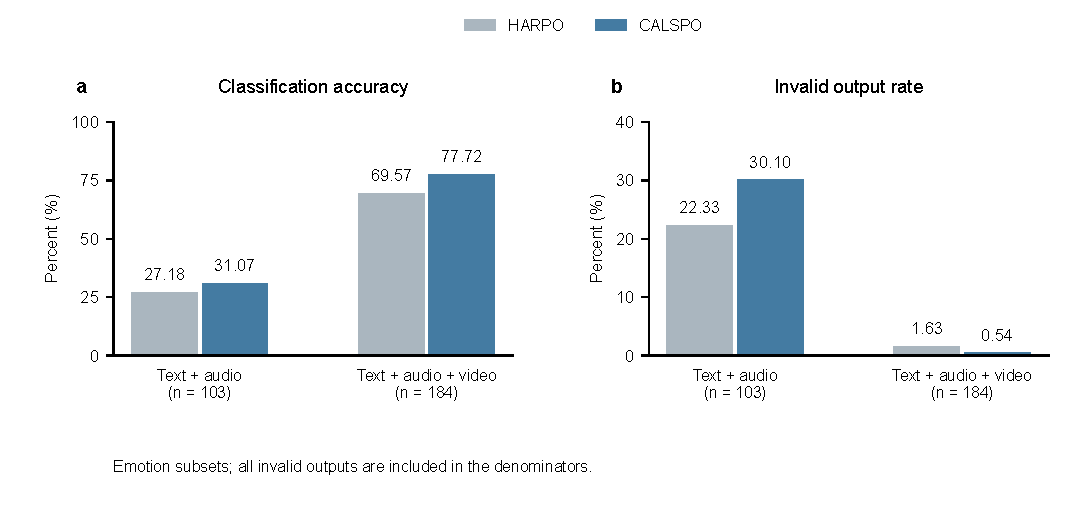
\includegraphics[width=\linewidth]{figures/fig3_modality.pdf}
\captionof{figure}{情绪分类的正确率与无效输出率。 a，正确率；b，无效输出率。文本与音频n=103，文本与视频与音频n=184。两种方法评估相同题目。各模态组来自不同样本，不构成在同题上移除视频的控制实验。}\label{fig:3}
\end{minipage}
\end{center}

\subsection{讨论与局限}

HARPO调节已有回答的优势幅值，AVSPO恢复塌缩组的更新方向，CALSPO进一步加入真实类别目标。这样的联合设计使策略更新与标签约束在同一过程内结合。本次比较显示，中性误判减少，情绪Macro-F1提高；同时，中性倾向及文本与音频输入中的格式问题仍然存在，预测分布的均衡性仍有改善空间。

当前比较包含优势恢复、标签监督、类别权重及任务层EMA变化，不能从整体结果单独确定各组件贡献。不同模态组的样本与类别构成亦不相同，模态差异不能直接归因于视频输入。组件消融及同题模态控制可进一步区分这些因素。模型选择中的评估信息复用可能引入选择偏差\cite{ref23}。本文结论限定于所报告的评估集；抑郁分类结果也仅反映标签匹配表现，不对应临床诊断能力。

\section{结论}

本文提出CALSPO，在HARPO策略优化中结合连续复合奖励下的优势恢复与类别加权标签监督，并训练得到EquiAffect-3B。方法实现与训练后LoRA权重共同构成本文的可复用产出。两个分类任务的比较显示，该联合配置提高了情绪分类指标，并降低非中性误判为中性的比例。与此同时，中性100\%召回对应的精确率仍有提升空间，文本与音频输入中的中性倾向与无效输出仍然存在。后续工作需要通过组件消融区分更新信号恢复、真实标签监督和频数权重的贡献，并进一步改善不同输入条件下的剩余偏向。

\clearpage
\begin{thebibliography}{99}
\small
\setlength{\itemsep}{4pt}
\bibitem{ref1} Shi T, Huang S L. \emph{MultiEMO: An Attention-Based Correlation-Aware Multimodal Fusion Framework for Emotion Recognition in Conversations}. ACL, 2023:14752–14766. \href{https://aclanthology.org/2023.acl-long.824/}{原文}.
\bibitem{ref2} Cheng Z, Cheng Z Q, He J Y, et al. \emph{Emotion-LLaMA: Multimodal Emotion Recognition and Reasoning with Instruction Tuning}. NeurIPS, 2024. \href{https://arxiv.org/abs/2406.11161v2}{原文}.
\bibitem{ref3} Ong K, Dai W, Li C, et al. \emph{Human Behavior Atlas: Benchmarking Unified Psychological and Social Behavior Understanding}. 2025. arXiv:2510.04899v1. \href{https://arxiv.org/abs/2510.04899v1}{原文}.
\bibitem{ref4} Lian Z, Chen H, Chen L, et al. \emph{AffectGPT: A New Dataset, Model, and Benchmark for Emotion Understanding with Multimodal Large Language Models}. 2025. arXiv:2501.16566v2. \href{https://arxiv.org/abs/2501.16566v2}{原文}.
\bibitem{ref5} Cui Y, Jia M, Lin T Y, Song Y, Belongie S. \emph{Class-Balanced Loss Based on Effective Number of Samples}. CVPR, 2019:9268–9277. \href{https://openaccess.thecvf.com/content_CVPR_2019/html/Cui_Class-Balanced_Loss_Based_on_Effective_Number_of_Samples_CVPR_2019_paper.html}{原文}.
\bibitem{ref6} Tu G, Jing R, Liang B, et al. \emph{A Training-Free Debiasing Framework with Counterfactual Reasoning for Conversational Emotion Detection}. EMNLP, 2023:15639–15650. \href{https://aclanthology.org/2023.emnlp-main.967/}{原文}.
\bibitem{ref7} Shao Z, Wang P, Zhu Q, et al. \emph{DeepSeekMath: Pushing the Limits of Mathematical Reasoning in Open Language Models}. 2024. arXiv:2402.03300v3. \href{https://arxiv.org/abs/2402.03300v3}{原文}.
\bibitem{ref8} Ong K, Boughorbel S, Xiao L, et al. \emph{OmniSapiens: A Foundation Model for Social Behavior Processing via Heterogeneity-Aware Relative Policy Optimization}. 2026. arXiv:2602.10635v2. \href{https://arxiv.org/abs/2602.10635v2}{原文}.
\bibitem{ref9} He X, Sun Q, Cheng A, et al. \emph{Advantage Collapse in Group Relative Policy Optimization: Diagnosis and Mitigation}. 2026. arXiv:2605.21125v2. \href{https://arxiv.org/abs/2605.21125v2}{原文}.
\bibitem{ref10} Yu Q, Zhang Z, Zhu R, et al. \emph{DAPO: An Open-Source LLM Reinforcement Learning System at Scale}. 2025. arXiv:2503.14476v1. \href{https://arxiv.org/abs/2503.14476v1}{原文}.
\bibitem{ref11} Nan G, Chen S, Huang J, et al. \emph{NGRPO: Negative-enhanced Group Relative Policy Optimization}. 2025. arXiv:2509.18851v1. \href{https://arxiv.org/abs/2509.18851v1}{原文}.
\bibitem{ref12} Chen P, Li X, Li Z, Chen X, Lin T. \emph{Stepwise Guided Policy Optimization: Coloring your Incorrect Reasoning in GRPO}. 2026. arXiv:2505.11595v5. \href{https://arxiv.org/abs/2505.11595v5}{原文}.
\bibitem{ref13} Ouyang L, Wu J, Jiang X, et al. \emph{Training language models to follow instructions with human feedback}. 2022. arXiv:2203.02155v1. \href{https://arxiv.org/abs/2203.02155v1}{原文}.
\bibitem{ref14} Fu Y, Chen T, Chai J, et al. \emph{SRFT: A Single-Stage Method with Supervised and Reinforcement Fine-Tuning for Reasoning}. 2025. arXiv:2506.19767v1. \href{https://arxiv.org/abs/2506.19767v1}{原文}.
\bibitem{ref15} Lin T Y, Goyal P, Girshick R, He K, Dollár P. \emph{Focal Loss for Dense Object Detection}. ICCV, 2017:2980–2988. \href{https://openaccess.thecvf.com/content_iccv_2017/html/Lin_Focal_Loss_for_ICCV_2017_paper.html}{原文}.
\bibitem{ref16} Menon A K, Jayasumana S, Rawat A S, Jain H, Veit A, Kumar S. \emph{Long-tail learning via logit adjustment}. ICLR, 2021. \href{https://arxiv.org/abs/2007.07314v2}{原文}.
\bibitem{ref17} Ren J, Yu C, Sheng S, et al. \emph{Balanced Meta-Softmax for Long-Tailed Visual Recognition}. NeurIPS, 2020. \href{https://papers.neurips.cc/paper_files/paper/2020/hash/2ba61cc3a8f44143e1f2f13b2b729ab3-Abstract.html}{原文}.
\bibitem{ref18} Tsai Y H H, Bai S, Liang P P, et al. \emph{Multimodal Transformer for Unaligned Multimodal Language Sequences}. ACL, 2019:6558–6569. \href{https://aclanthology.org/P19-1656/}{原文}.
\bibitem{ref19} Xu J, Guo Z, He J, et al. \emph{Qwen2.5-Omni Technical Report}. 2025. arXiv:2503.20215v1. \href{https://arxiv.org/abs/2503.20215v1}{原文}.
\bibitem{ref20} Hu E J, Shen Y, Wallis P, et al. \emph{LoRA: Low-Rank Adaptation of Large Language Models}. 2021. arXiv:2106.09685v2. \href{https://arxiv.org/abs/2106.09685v2}{原文}.
\bibitem{ref21} Schulman J, Wolski F, Dhariwal P, Radford A, Klimov O. \emph{Proximal Policy Optimization Algorithms}. 2017. arXiv:1707.06347v2. \href{https://arxiv.org/abs/1707.06347v2}{原文}.
\bibitem{ref22} Loshchilov I, Hutter F. \emph{Decoupled Weight Decay Regularization}. ICLR, 2019. \href{https://arxiv.org/abs/1711.05101v3}{原文}.
\bibitem{ref23} Cawley G C, Talbot N L C. \emph{On Over-fitting in Model Selection and Subsequent Selection Bias in Performance Evaluation}. Journal of Machine Learning Research, 2010, 11(70):2079–2107. \href{https://jmlr.org/papers/v11/cawley10a.html}{原文}.
\bibitem{ref24} Sheng G, Zhang C, Ye Z, et al. \emph{HybridFlow: A Flexible and Efficient RLHF Framework}. 2024. arXiv:2409.19256v2. \href{https://arxiv.org/abs/2409.19256v2}{原文}.
\bibitem{ref25} Wang S, Guðnason J, Borth D. \emph{Learning Emotional Representations from Imbalanced Speech Data for Speech Emotion Recognition and Emotional Text-to-Speech}. Interspeech, 2023:351–355. DOI:10.21437/Interspeech.2023-1595. \href{https://www.isca-archive.org/interspeech_2023/wang23ka_interspeech.html}{原文}.
\end{thebibliography}
\clearpage
\appendix
\section{算法与实现细节}

\subsection{CALSPO训练流程}

\textbf{算法1｜类别感知监督策略优化。} 输入为带任务与真实标签的训练问题、策略参数、训练类别权重及历史阈值与EMA状态；输出为更新后的策略参数。

\begin{enumerate}
\item 为每个问题生成G=4个真实回答，计算正确性、格式与长度复合奖励。
\item 在当前批全部真实回答上进行奖励归一化，计算各问题的组内总体标准差及批次塌缩率。
\item 根据当前阈值判断优势恢复是否触发；仅为满足奖励塌缩且全对或全错的组构造虚拟奖励。
\item 利用真实与虚拟奖励的联合统计，仅计算真实回答优势；其余组使用原有奖励统计。
\item 从真实优势幅值计算问题尺度与任务尺度，更新任务层EMA状态，得到最终优势。
\item 对真实采样回答计算裁剪策略损失。
\item 按问题唯一标识去重，为每个问题构造真实标签及结束符目标。
\item 计算类别加权的辅助损失，与策略损失共同更新LoRA参数。
\item 根据原始奖励均值的批间变化更新动态阈值，用于下一批触发判断。
\end{enumerate}

\subsection{复合奖励归一化与优势恢复}

对真实回答i，原始奖励为：

\begin{equation*}
R_i=0.8y_i+0.2f_i+0.75p(L_i)
\end{equation*}

其中，$y_i$表示最终标签是否与真实标签一致；$f_i$表示是否满足实现规定的思考段与方框答案格式；$L_i$为分词后的回答长度。长度项在$L_i$$\le$192时为0，在192<$L_i$$\le$256时为(192$-$$L_i$)/64，超过256时为$-$1。该项用于限制过长回答，不能解释为推理质量评分。

在当前训练批全部真实回答上进行最小—最大归一化：

\begin{equation*}
r_i=\frac{R_i-R_{\min}}{\max(R_{\max}-R_{\min},\varepsilon)},\qquad\varepsilon=10^{-6}
\end{equation*}

归一化范围为整个批次，而非单个问题组。由于格式和长度也参与奖励，答案全部错误或全部正确，并不必然意味着组内奖励塌缩。因此，后续分别检查奖励方差和答案正确性。

对问题q，以G个归一化奖励的总体标准差判断组内塌缩：标准差低于$10^{-6}$时，将该组记为塌缩组。批次塌缩率ACR为塌缩问题数占本批问题数的比例。当ACR超过动态阈值$\theta$，且某组同时满足奖励塌缩与全部回答错误或全部回答正确时，才为该组加入虚拟奖励统计。阈值初值为0.1。

虚拟奖励数设置为：

\begin{equation*}
K=\operatorname{clip}\!\left(\left\lceil G\,\mathrm{ACR}^{0.5}\right\rceil,\,1,\,G\right)
\end{equation*}

以塌缩组首个真实奖励$r_0$为锚点，虚拟锚距尺度h=0.1。对于全错组，j=0,…,K$-$1时，虚拟奖励为$r_0$+h(K$-$j)/K；对于全对组，为$r_0$$-$h(j+1)/(K+1)。将真实奖励与虚拟奖励合并计算均值$\mu_{\mathrm{aug}}$和总体标准差$\sigma_{\mathrm{aug}}$，再仅对G个真实回答计算：

\begin{equation*}
a_i=\frac{r_i-\mu_{\mathrm{aug}}}{\max(\sigma_{\mathrm{aug}},\varepsilon)}
\end{equation*}

未触发虚拟奖励的组使用原有G个真实奖励计算相同形式的标准化优势。对于全错塌缩组，较高的虚拟奖励使真实回答获得负优势；对于全对塌缩组，较低的虚拟奖励使真实回答获得正优势。这一构造改变了组内参照，却没有在原本等价的真实回答间制造优劣排序。因此，它提供恢复后的更新方向，并不保证模型自动生成正确标签或更有区分度的答案。

动态阈值在当前批完成触发判断后更新。设$\Delta$为本批与上一批原始奖励均值之差，学习系数$\eta$=0.01，则$\theta_{\mathrm{next}}$=clip[$\theta$+$\eta$·sign($\Delta$)·(ACR$-$$\theta$),0,1]。首批仅建立历史奖励均值。

\subsection{HARPO调制的本地实现}

CALSPO以|$a_i$|作为贡献代理量，在同一任务内调节问题尺度，再在本批出现的任务之间调节任务尺度。对问题q，令$u_q$=max($\operatorname{mean}_i$|$a_i$|,$\varepsilon$)，同任务问题的几何均值为$g_m$，则问题尺度为：

\begin{equation*}
s_q=\operatorname{clip}\!\left(\frac{g_m}{u_q},\,0.5,\,3.0\right)
\end{equation*}

问题层尺度由当前批次计算，不跨批次进行指数移动平均；任务内只有一个问题时，该尺度为1。

任务层先按每个任务的真实回答数，计算绝对优势均值$\rho_m$。在$\varepsilon$下界保护下，对$\rho_m$使用指数移动平均（exponential moving average，EMA），前一状态与当前值的系数分别为0.75和0.25；任务密度与任务对数尺度的状态均从0初始化，因此首次更新的密度为当前批密度的0.25倍。在本批出现的任务中计算平滑密度的几何均值$g_\rho$，得到瞬时对数尺度log($g_\rho$/$\rho_{m,\mathrm{EMA}}$)。再以同样的0.75/0.25系数平滑对数尺度，指数变换后截断至[0.5,4.0]。最终优势为：

\begin{equation*}
A_i=a_i\,s_q\,s_m
\end{equation*}

同一回答的有效生成token共享该优势。任务层参照仅包含当前批出现的任务，并不在每一步对所有训练任务进行全局比较。

\subsection{标签目标与类别权重}

标签监督旨在补充真实类别的直接学习目标。按问题唯一标识对G个回答去重，保留每个原始问题一次，使用相同多模态输入，构造“方框中的真实标签＋序列结束符”作为教师强制目标。该目标没有思考段，也没有推理过程监督。使用快速分词器的字符偏移识别标签内容token：只要token与标签字符区间存在重叠，即归入标签内容；其余目标中的有效token归入格式及结束符部分。

设$L_{\mathrm{label}}$为标签内容token的平均负对数似然，$L_{\mathrm{format}}$为格式与结束符token的平均负对数似然，则：

\begin{equation*}
L_{\mathrm{target}}(q)=L_{\mathrm{label}}(q)+0.5L_{\mathrm{format}}(q)
\end{equation*}

类别权重仅由训练集计算。任务m共有$N_m$个训练问题、$C_m$类，第c类频数为$n_{mc}$，原始权重为sqrt[$N_m$/(|$C_m$|$n_{mc}$)]。用该任务内按样本频数加权的原始权重均值$Z_m$归一化，再截断至[0.5,2.0]，得到$w_{mc}$。截断后不进行二次归一化。最终辅助损失为：

\begin{equation*}
L_{\mathrm{aux}}=\frac{1}{Q}\sum_q w_{mc}L_{\mathrm{target}}(q)
\end{equation*}

其中Q为当前PPO minibatch内去重后的问题数，本次为8。这里对问题数取平均，既不对4倍回答数取平均，也不除以权重总和。本次训练集的情绪中性类包含64/224个问题，其标签权重为0.7204；其余情绪类别权重为1.0188至1.3222。权重根据训练频数确定，不随模型当前预测分布动态改变。

\begingroup
\small
\setlength{\tabcolsep}{4pt}
\renewcommand{\arraystretch}{1.22}
\begin{longtable}{>{\raggedright\arraybackslash}p{\dimexpr 0.22\linewidth-7.04pt\relax}>{\raggedright\arraybackslash}p{\dimexpr 0.25\linewidth-8.0pt\relax}>{\raggedright\arraybackslash}p{\dimexpr 0.25\linewidth-8.0pt\relax}>{\raggedright\arraybackslash}p{\dimexpr 0.28\linewidth-8.96pt\relax}}
\toprule
\textbf{任务} & \textbf{类别} & \textbf{训练频数} & \textbf{标签监督权重} \\
\midrule
\endfirsthead
\toprule
\textbf{任务} & \textbf{类别} & \textbf{训练频数} & \textbf{标签监督权重} \\
\midrule
\endhead
\bottomrule
\endfoot
情绪 & 愤怒 & 19 & 1.3222 \\
情绪 & 厌恶 & 27 & 1.1091 \\
情绪 & 恐惧 & 26 & 1.1303 \\
情绪 & 高兴 & 32 & 1.0188 \\
情绪 & 中性 & 64 & 0.7204 \\
情绪 & 悲伤 & 24 & 1.1764 \\
情绪 & 惊讶 & 32 & 1.0188 \\
抑郁分类 & 抑郁 & 17 & 1.6088 \\
抑郁分类 & 非抑郁 & 63 & 0.8357 \\
\end{longtable}
\endgroup

\subsection{策略损失与计算范围}

总损失为L=$L_{\mathrm{policy}}$+$\lambda$$L_{\mathrm{aux}}$，本次$\lambda$=1.0。策略损失以PPO式裁剪目标为基础\cite{ref21}。对每个有效生成token计算新旧策略的条件概率比，对数比先截断至[$-$20,20]；常规概率比裁剪范围为[0.8,1.2]，负优势使用系数3.0的dual-clip处理。实现先按每个回答的有效生成token求均值，再在回答间求均值。一个包含8个原始问题的训练批产生32个强化学习回答，同时包含8个标签监督目标。

两类损失在同一优化流程中累积梯度。标签监督需要额外的教师强制前向和反向计算，不应被描述为无计算成本。当前配置不使用奖励KL项、策略KL损失或熵正则，也不训练独立critic。

现有资源记录未提供匹配条件下的完整训练成本比较。辅助标签监督增加教师强制前向与反向计算，具体训练时间、显存及资源代价需由对应实测记录确定。

\section{数据与实验设置}

\subsection{数据构成}

本研究选取Human Behavior Atlas\cite{ref3}中的情绪分类与抑郁分类任务进行实验。训练集包含304个问题，其中情绪分类224题、抑郁分类80题；按输入模态划分，文本80题、文本与音频152题、文本与视频与音频72题。情绪训练标签中，中性64题，愤怒19题、厌恶27题、恐惧26题、高兴32题、悲伤24题、惊讶32题。抑郁分类包含抑郁17题、非抑郁63题。辅助类别权重完全由上述训练频数确定。

本文使用提供的328题评估集进行比较，其中情绪分类287题、抑郁分类41题；情绪七类各41题，抑郁与非抑郁分别为11题和30题。输入包含文本与视频与音频184题、文本与音频103题和纯文本41题。纯文本均对应抑郁分类，因此模态比较与任务分布存在关联，不能将纯文本与其他模态的指标直接解释为单一模态效应。

\subsection{训练与推理参数}

\begingroup
\small
\setlength{\tabcolsep}{4pt}
\renewcommand{\arraystretch}{1.22}
\begin{longtable}{>{\raggedright\arraybackslash}p{\dimexpr 0.26\linewidth-4.16pt\relax}>{\raggedright\arraybackslash}p{\dimexpr 0.74\linewidth-11.84pt\relax}}
\toprule
\textbf{项目} & \textbf{本研究设置} \\
\midrule
\endfirsthead
\toprule
\textbf{项目} & \textbf{本研究设置} \\
\midrule
\endhead
\bottomrule
\endfoot
基座模型 & Qwen2.5-Omni-3B \\
训练形式 & 单模型联合训练情绪分类与抑郁分类；HARPO作为基线，CALSPO采用联合优化目标 \\
实现框架 & VERL／HybridFlow\cite{ref24} \\
训练长度 & 38个训练步 \\
学习率 & 1$\times$$10^{-6}$ \\
优化器 & AdamW\cite{ref22} \\
每题回答数 & 4 \\
有效批大小 & 8个问题，对应32条采样回答 \\
PPO minibatch & 8个问题，对应32条采样回答 \\
提示／回答长度上限 & 1536／256 token \\
任务层惯性平滑系数 & HARPO的两项旧值系数均为0.95；CALSPO均为0.75 \\
KL正则 & 省略显式KL奖励与KL损失 \\
奖励 & 正确性、格式与长度惩罚的组合，见第3.4节 \\
\end{longtable}
\endgroup

LoRA作用于q、k、v、o及gate、up、down投影，秩为16，lora\_alpha为32。训练采用单张P40 GPU；LoRA可训练参数保存为float32，计算采用float16混合精度。评估采用贪心解码，每题生成一个回答。

\subsection{指标定义}

正确率为合法且正确的预测占全部评估问题的比例；无效输出率为未匹配合法标签的答案占比。每类精确率P=TP/(TP+FP)，召回率R=TP/(TP+FN)，F1=2PR/(P+R)。Macro-F1对任务内合法类别的F1取等权平均；无效答案作为其真实类别的漏判保留，不作为额外真实类别参与平均。表中F1值乘以100显示。

中性误判率以全部真实非中性问题为分母；中性预测占比以相应范围全部问题为分母；中性召回以真实中性问题为分母。输出文本诊断另统计提取答案是否以“neutral”开头，该比例不改变严格标签判定。

\section{分模态补充结果}


\begingroup
\small
\setlength{\tabcolsep}{4pt}
\renewcommand{\arraystretch}{1.22}
\renewcommand{\thetable}{C\arabic{table}}
\setcounter{table}{0}
\begin{longtable}{>{\raggedright\arraybackslash}p{\dimexpr 0.333\linewidth-8.0pt\relax}>{\raggedright\arraybackslash}p{\dimexpr 0.333\linewidth-8.0pt\relax}>{\raggedright\arraybackslash}p{\dimexpr 0.333\linewidth-8.0pt\relax}}
\caption{分模态Macro-F1（\%）。 各值在相应任务合法类别上等权平均，保留无效答案产生的漏判。}\label{tab:C1}\\
\toprule
\textbf{输入与任务} & \textbf{HARPO Macro-F1} & \textbf{CALSPO Macro-F1} \\
\midrule
\endfirsthead
\toprule
\textbf{输入与任务} & \textbf{HARPO Macro-F1} & \textbf{CALSPO Macro-F1} \\
\midrule
\endhead
\bottomrule
\endfoot
文本＋音频／情绪 & 20.92\% & 26.11\% \\
文本＋视频＋音频／情绪 & 66.85\% & 76.01\% \\
文本／抑郁 & 96.80\% & 96.80\% \\
\end{longtable}
\endgroup

\section{数据与代码可用性草案}

本研究的方法实现、训练与评估数据、两组消融代码及EquiAffect-3B训练后LoRA权重归档于\href{https://github.com/zhe293/CALSPO}{CALSPO仓库}，当前为私有仓库。EquiAffect-3B适配权重对应第38步检查点，包含权重文件、适配器配置及SHA-256校验记录；基座为Qwen/Qwen2.5-Omni-3B，固定版本为f75b40e3da2003cdd6e1829b1f420ca70797c34e，基座权重通过官方下载入口获取。模型使用时需将基座与适配权重共同加载。图表来源数据、绘图脚本及核对记录与初稿一并保存。仓库计划在终版投稿时转为公开，原始数据与基座的分享范围遵照各自来源许可。
\end{document}
